%%% !TEX TS-program = PartialThesis

%%% Most settings such as pagesize controls are hidden 
%%% in the apithesis.cls, which also imports a host of
%%% helpful packages.
%%% 
%%% Special options are:
%%%   - final / draft
%%%   - cropmarks / nocropmarks
%%%   - frame / noframe
%%%   - print / noprint
%%% Because apithesis is a specialized book class, you can
%%% also use regular options such as [fleqn, opeany] etc.
%%% 
%%% In draft mode the document is typeset using B5 page margins
%%% on a A4 page size.
%%% In final mode the document is typeset using B5 page size,
%%% while frames and/or cropmarks will be removed.
%%%
% \documentclass[fleqn,draft,noframe,cropmarks]{styles/apithesis}
\documentclass[final,print]{styles/apithesis}
\usepackage{graphicx}
\usepackage[varg]{txfonts}
\usepackage{amsmath}
%\usepackage[dvipsnames]{xcolor}
\usepackage{comment}
\usepackage{multirow}
\usepackage{url}
\usepackage[normalem]{ulem}
\usepackage{epsfig}
\usepackage{amsmath}
\usepackage{amsfonts}
\usepackage{amssymb}
\usepackage{listings}
%%% for tree diagram
\usepackage{forest}
\usepackage{tikz-qtree}
\usetikzlibrary{shadows,trees}
\usepackage{lscape}
\usepackage[utf8]{inputenc}
\usepackage[T1]{fontenc}
\usepackage{wrapfig}
\usepackage{supertabular}
\usepackage[scientific-notation=true]{siunitx}

%%% Load your customized layout file
% !TEX root =  thesis.tex

% This document describes all layout settings for page headings, section titles,
% linespread etcetera.

%----------------------------------------------------------------------------------------
%	CONTROL PACKAGES
%----------------------------------------------------------------------------------------

\usepackage[titletoc]{appendix}	% for additional appendix formatting commands
%\usepackage[Bjornstrup]{fncychap}		% for chapter symbol formatting
\usepackage{titletoc}
\usepackage[nottoc]{tocbibind}	% Add the bibliography to the table of content
\usepackage{titlesec}
\usepackage{fancyhdr}
\usepackage[footnotesize,bf]{caption}	% change caption formatting
\usepackage{pdfpages}

%----------------------------------------------------------------------------------------
%	TYPEFACE SETTINGS
%----------------------------------------------------------------------------------------

% A selection of font packages
%\usepackage{mathpazo}				% Adds palatino like math symbols
%\usepackage{helvet}				% Use helvetica as main fonts
%\usepackage[charter]{mathdesign} 	% Use 'Adobe Utopia' as math font
%\usepackage[garamond]{mathdesign} 	% Use 'URW Gara?mond' as math font
%\usepackage[utopia]{mathdesign} 	% Use 'Bit?stream Char?ter' as math font
%\usepackage{txfonts}				% Use 'Times'-line math font
%\newcommand\hmmax{0}\usepackage{bm}% Add bold font math symbols
%\usepackage[mathcal]{eucal}		% Use the 'Euler' math font


% Mix-n-match your preferred thesis font
\DeclareSymbolFont{usualmathcal}{OMS}{cmsy}{m}{n}			% set symbol font
\DeclareSymbolFontAlphabet{\mathcal}{usualmathcal}			% set calligraphic math symbols
\DeclareMathAlphabet{\mathbbm}{U}{bbm}{m}{n}				% set bold math font

%----------------------------------------------------------------------------------------
%	SPACING SETTINGS
%----------------------------------------------------------------------------------------

% Set spacing options
\linespread{1.1}
\addtolength{\footskip}{0.5cm}
\addtolength{\headheight}{\baselineskip}

\interfootnotelinepenalty=10000

%\addtolength{\headheight}{1.1pt}

%\setlength{\captionmargin}{4mm}

\renewcommand{\contentsname}{Contents}
\setcounter{tocdepth}{1}

\fnbelowfloat % place bottom float above the footnotes


%%%%%%%%%%%%%%%%%%%%%%%%
%\setlength{\parindent}{0cm}
\addtolength{\voffset}{1.5\baselineskip}
\addtolength{\evensidemargin}{-10mm}
\addtolength{\oddsidemargin}{10mm}

%\renewcommand{\sectfont}{\rmfamily\bfseries}
\addto\captionsenglish{\renewcommand{\figurename}{\footnotesize Fig.}}
\renewcommand{\topfraction}{0.9}  % Florian: 0.9
\renewcommand{\bottomfraction}{0.9}  % Florian: 0.9
\renewcommand{\textfraction}{0.1}
\renewcommand{\floatpagefraction}{0.8}
\setlength{\floatsep}{14pt plus 10pt minus 4pt}
\setlength{\intextsep}{14pt plus 10pt minus 4pt}
\setlength{\textfloatsep}{20pt plus 12pt minus 4pt}


%%%%%%%%%%%%%%%%%%%%%%%%%%%%%%%%%%%%%%%%%%%%%%%%%%%%%%%%%%%%%%%%%%%%%%%%%%%%%%%%
%USE:
%  Here's where the tabletoc and titlesec stuff is put.
%\titleformat{cmd}[shape]{format}{label}{sep}{before-code}
%{cmd} = \chapter, \section etc.
%[shape]: 'display' puts the title chapter on a separate line, 'hang' a hanging label (label begint op zelfde regel als nummer en gaat eronder door), 'runin' should produce a run-in title, but that is not working, 'frame' puts a line-frame around the title.
%{format}: typeset, applies to both label and text
%{label}: formatting of the heading (chapter) number, refer to actual number by using \thechapter
%{sep}: distance between heading number and title text. Depending on the shape argument this can refer either to vertical or horizontal spacing
%{before-code}: code executed preceding the heading text, picks up heading text
%
%\titlespacing{cmd}{left-sep}{before-sep}{after-sep}[rigth-sep]
%{left-sep}: specifies the increase in the left margin
%{before-sep}: vertical space added above the heading
%{after-sep}: seperation between heading and following paragraph
%[rigth-sep]: specifying increase in right margin


% %   Mathieu Renzo 
% \titleformat{\chapter}[display]
% {\huge}
% {\vspace*{-2.4\baselineskip}\raggedright
%   \textcolor{gray!50}{\hspace*{15pt}{\normalsize\chaptertitlename}}\\\titlerule\vspace*{0.5pc}\hspace*{-5pt}\textcolor{gray!50}{\fontsize{160}{160}\selectfont\thechapter}\titlerule\vspace*{1pc}}
% {-95pt}{\sffamily \slshape \hspace*{90pt}\parbox[t][0pt][c]{0.79\textwidth}}
% \titlespacing{\chapter}{0pt plus 0pt minus 100pt}{0pt plus 3pt minus 3pt}{60pt plus 10pt minus 50pt}

%% load font
% \usepackage{metrouberfont}

\titleformat{\chapter}[display]{\LARGE}{\vspace*{-2.3\baselineskip}\raggedleft\textcolor{chcol}{\normalsize\rm
    \chaptertitlename\hspace*{2.5em}}\\\titlerule\vspace*{0.5pc}{\hrulefill\fontsize{150}{150}\selectfont\selectfont\textcolor{chcol}{\thechapter}}}{-77pt}{
  \scshape \rmfamily \linespread{1000}\parbox[t][0pt][c]{0.8\textwidth}}
\titlespacing{\chapter}{0pt plus 0pt minus 100pt}{0pt plus 3pt minus 3pt}{80pt
  plus 60pt minus 50pt}

\titleformat{\section}
 {\normalfont\Large\bfseries}{\thesection}{1em}{}

\titleformat{\subsection}
 {\normalfont\large\bfseries}{\thesubsection}{1em}{}

\titleformat{\subsubsection}
 {\normalfont\normalsize\bfseries}{\thesubsubsection}{1em}{}


%%%%%%%%%%%%%%%%%%%%%%%%%%%%%%%%%%%%%%%%%%%%%%%%%%%%%%%%%%%%%%%%%%%%%%%%%%%%%%%%


% This is to get completely empty pages on the left of a chapter opening page.
\makeatletter
\def\cleardoublepage{\clearpage\if@twoside \ifodd\c@page\else
  \hbox{}
  \thispagestyle{plain}
  \newpage
  \if@twocolumn\hbox{}\newpage\fi\fi\fi}
\makeatother
%%%%%%%%%%%%%%%%%%%%%%%%%%%%%%%%%%%%%%%%%%%%%%%%%%%%%%%%%%%%%%%%%%%%%%%%%%%%%%%%
%  fancyhdr settings

\pagestyle{fancy}


%THESE COMMANDS GET THE CHAPTER HEADER AND NUMBER
%\renewcommand{\chaptermark}[1]{\markboth{
%  \sffamily \small \bfseries \chaptertitlename\ \thechapter:\ #1}{}}
\renewcommand{\chaptermark}[1]{\markboth{
    \rm \small \scshape\thechapter \; \ #1 }{}}
\renewcommand{\headrulewidth}{0.5pt}
\newcommand{\chapsubhead}[1]{{\normalsize #1}}%
  
\renewcommand{\sectionmark}[1]{\markright{
  \rm \small \scshape  \thesection  \; \ #1 }}

% Chapter title on the left, paragraph on the right.
% Page numbers on the outside.
%\fancyhf[HLE]{\nouppercase{\leftmark}}
%\fancyhf[HRO]{\nouppercase{\rightmark}}
%\fancyhf[HLO]{\thepage}
%\fancyhf[HLE]{\thepage}
% -----
\fancyhf{}
%\fancyhead[LE]{\leftmark}
%\fancyhead[RO]{\rightmark}

\fancyhead[LE]{\nouppercase{\leftmark}}
\fancyhead[RO]{\nouppercase{\rightmark}}

\fancyfoot[LE,RO]{\small\thepage}
\fancyfoot[C]{}

% for the chapter opening pages:
\fancypagestyle{plain}{    
  \fancyhf{}
  \fancyfoot[C]{}
  \renewcommand{\headrulewidth}{0pt}
  \fancyfoot[LE,RO]{\small\thepage}
}

\setlength{\parskip}{0pt}

%%%%%%%%%%%%%%%%%%%%%%%%%%%%%%%%%%%%%%%%%%%%%%%%%%%%%%%%%%%%%%%%%%%%%%%%%%%%%%%%

% Custom environment definitions
\newenvironment{abstract}
{\begin{center}{\it\normalsize Abstract}\\ \end{center}}
{\clearpage}

\newcommand{\chauthors}[1]{\begin{center} {\rm\normalsize #1} \\ \end{center}}
\newcommand{\chjournal}[1]{\begin{center} {\it\normalsize #1} \\ \medskip \end{center}}

%%%%%%%%%%%%%%%%%%%%%%%%%%%%%%%%%%%%%%%%%%%%%%%%%%%%%%%%%%%%%%%%%%%%%%%%%%%%%%%%


%\rfoot{\setlength{\unitlength}{1mm}
%\begin{picture}(5,0)
%\put(5,0){\includegraphics[width=3cm]{ok/expo000\thepage.epsi}}
%\end{picture}}

%%%%%%%%%%%%%%%%%%%%%%%%%%%%%%%%%%%%%%%%%%%%%%%%%%%%%%%%%%%%%%%%%%%%%%%%%%%%%%%%



%%% Local Variables:
%%% mode: latex
%%% TeX-master: "../thesis_renzo"
%%% End:


%%% Load your custom latex commands
% !TEX root =  thesis.tex

%----------------------------------------------------------------------------------------
%	CUSTOM COMMANDS
%----------------------------------------------------------------------------------------

% Define all you customized latex commands hereo

% Define a command for a partial derivative (curly d's)
% Use as:
%   \partial{x}{t}      => dx / dt
%   \partial[n]{x}{t}   => d^n x / dt^n
%
\newcommand{\deriv}[3][1]{%
	\ifthenelse{\equal{#1}{1}}{		% true: format without power
		\ensuremath{\frac{\partial#2}{\partial#3}}
	}{								% false: format with power
		\ensuremath{\frac{\partial^{#1}#2}{\partial#3^{#1}}}
	}%
}

% Unit shortcuts
\newcommand{\um}{\ensuremath{\mu \rm{m}}\xspace}
\newcommand{\degr}{\ensuremath{^{\circ}}\xspace}
\newcommand{\arcsec}{\ensuremath{^{\prime\prime}}\xspace}

% Scientific notation short cut
\newcommand{\E}[1]{\ensuremath{\times10^{#1}}}
\newcommand{\pair}{\ensuremath{e^\pm}}
\newcommand{\udef}{\stackrel{\mathrm{def}}{=}}
\newcommand{\kms}{{\mathrm{km\ s^{-1}}}}
\newcommand{\Msun}{{\mathrm{M}_\odot}}
\newcommand{\masyr}{\,\mathrm{mas}\,\mathrm{yr}^{-1}}

% A few commands that control brackets
\newcommand{\sbr}[1]{\ensuremath{\left\{ #1 \right\}}}
\newcommand{\cbr}[1]{\ensuremath{\left( #1 \right)}}
\newcommand{\rbr}[1]{\ensuremath{\left[ #1 \right]}}

% Miscellanea
\DeclareRobustCommand{\Eqref}[1]{Eq.~\ref{#1}}
\DeclareRobustCommand{\Figref}[1]{Fig.~\ref{#1}}
\DeclareRobustCommand{\Tabref}[1]{Tab.~\ref{#1}}
\DeclareRobustCommand{\Secref}[1]{Sec.~\ref{#1}}
\DeclareRobustCommand{\Chref}[1]{Ch.~\ref{#1}}

\newcommand{\binaryc}{\texttt{binary\_c}\ }

\definecolor{Orange}{HTML}{FF9900}
\newcounter{TODOLIST}
\newcommand{\todo}[1]{\stepcounter{TODOLIST} {$\blacksquare$~\textbf{\color{red}[TODO: #1]}}~$\blacksquare$}
\renewcommand{\labelitemii}{$\bullet$}


% citation aliases
\defcitealias{tauris:98}{TT98}
\defcitealias{ramirez-agudelo:15}{R-A15}

\interfootnotelinepenalty=10000    % brute-forces the footnote not to break over two pages
\setlength{\belowcaptionskip}{-5pt}

%%% TOC customization%%% TOC customization
\makeatletter
\renewcommand{\@dotsep}{10000} 
\makeatother
%%% Local Variables:
%%% mode: latex
%%% TeX-master: "../thesis_renzo"
%%% End:


%%% Prepare the title page information
\title{your title}
\author{Your name}
\date{date,te 11:00\,uur}  %% make sure this is in dutch
\location{Aula der Universiteit}


%%%------------------------------------------------------------------------------------------
%%%	FRONTMATTER
%%%------------------------------------------------------------------------------------------
%%% limit compilation time by compiling only what you need
%%% \includeonly{content/intro/intro} 

\begin{document}
\frontmatter
% !TEX root =  thesis.tex

%
% The mandatory, pedel-approved title page (front/back)
%

% Change global settings, but restore them at the end!
\pagestyle{empty}
\setlength\parindent{0pt}

% Parse the title information to the pdf meta data
\makeatletter
\hypersetup{%
    pdftitle={\@title},
    pdfauthor={\@author},
    pdfsubject={Astronomy},
    pdfcreator={\@author}}
\makeatother


%----------------------------------------------------------------------------------------
%	COVER PAGE
%----------------------------------------------------------------------------------------

% Use a bit of minipage trickery to shift the title page to the center
%\begin{minipage}[c][190mm][c]{118mm} %% Full center
\begin{minipage}[c][190mm][c]{124mm}  %% 6mm offset from center to right
% For the print edition I choose to offset the page to compensate for the
% binding back. This gives the illusion that the title page is centered.
% For the digital edition I use the true center. 
\makeatletter
\begin{center}
	%% Leading whitespace
	\vspace*{1.2cm}

	%% Thesis title
	{ \huge \bf \@title }\\[2.7cm]

	%% Thesis type
	\textsc{\Large ACADEMISCH PROEFSCHRIFT}\\[1.2cm]
	\ifdraft \textsc{\Large DRAFT -- \today}\\[1.0cm] \fi
	
	%% Auxiliary details
	\linespread{1.2}
	\large \textrm{
		ter verkrijging van de graad van doctor \\
		aan de Universiteit van Amsterdam \\
		op gezag van de Rector Magnificus \\
		prof.~dr.~K.~I.~J.~Maex \\
		ten overstaan van een door het College voor Promoties ingestelde \\
		commissie, in het openbaar te verdedigen in de \@location \\
		op \@date \\ 
		\vspace{0.9cm}
		door \\[0.3cm]
		\vspace{0.9cm}
		{\bf \@author}\\[0.3cm]
 		geboren te BIRTHPLACE \\[0.3cm]  
	 }
\end{center}
\makeatother
\end{minipage}

%% Clear out the remaining page
\clearpage


%----------------------------------------------------------------------------------------
%	DOCTORAL BOARD
%----------------------------------------------------------------------------------------

% Custom header type
{\bf\normalsize Promotiecommissie:} \\[0.2cm]

% List boardmembers
\begin{tabular}{@{}lll}
     Promotor:      & prof.~dr.   & Universiteit van Amsterdam\\
					&									&	                         \\
	Overige leden:	&  & \\
                    &  & \\
                    &  & \\
                    &  & \\
                         
                    &  & \\
                    &  & \\
                    &  &

\end{tabular} 

\vspace*{0.2cm}
% Note faculty
Faculteit der Natuurwetenschappen, Wiskunde en Informatica

% Optional footnote
\vspace*{\fill}

\begin{figure}[!h]

\includegraphics[width=0.4\textwidth]{gfx/titlepage/UvA_logo.pdf}
\hspace{4cm}

\includegraphics[width=0.25\textwidth]{gfx/titlepage/API_logo.pdf}
\end{figure}

% Report financial backing of the research (see article 15.5)
{\small The research reported in this thesis was carried out at the Anton
  Pannekoek Institute for Astronomy (API), University of Amsterdam. It was supported by fundings from the National Science
  Foundation under Grant No.~NSF PHY11-25915. The Leids Kerkhoven-Bosscha Fonds
  (LKBF) provided occasional travel fundings.} \vspace{0.5em}

\clearpage

\thispagestyle{empty}
\null\vfill\null
\hfill\parbox{110mm}{
  \raggedleft
    \emph{\large quote}\\[5pt]
  S.~omeone
}
\null\vfill\null
\clearpage
\thispagestyle{empty}
\newpage
\phantom{let's kill those trees}

%----------------------------------------------------------------------------------------
%   Restore default settings
%----------------------------------------------------------------------------------------
\pagestyle{fancy}
\setlength\parindent{15pt}


%%% Local Variables:
%%% mode: latex
%%% TeX-master: "../thesis_renzo"
%%% End:
 	%%% mandatory 

%%%---------------------------------------------------------------------------------------
%%%	LIST OF CONTENTS
%%%------------------------------------------------------------------------------------------

% !TEX root =  thesis.tex

% PAGE HEADINGS
\pagenumbering{roman}%\setcounter{page}{1}
\cleardoublepage
\fancyhead[LE,RO]{\rmfamily \small \scshape \contentsname}
\fancyhead[LO,RE]{}


%%%% table of contents %%%%
{
  \hypersetup{linkcolor=chcol}
  \tableofcontents
}
%\listoffigures
%\listoftables
\cleardoublepage
% \clearpage
% restore page numbering style 
\setcounter{page}{1}
\pagenumbering{arabic}

\fancyhead[LE]{\leftmark}
\fancyhead[RO]{\rightmark}

%%% Local Variables:
%%% mode: latex
%%% TeX-master: "../thesis_renzo"
%%% End:
 			%%% Table of content
% \newpage
% \phantom{let's kill those tree!}
%%%------------------------------------------------------------------------------------------
%%%	THESIS CHAPTERS
%%% ------------------------------------------------------------------------------------------
\setcounter{page}{1}        	%%%\cleardoublepage
\mainmatter
\chapter{Introduction}
\label{ch:intro}

\graphicspath{{./gfx/fig_intro/}}


\section{Section}
\label{ch_intro:sec1}


\begin{figure}[tbp]
  \centering
  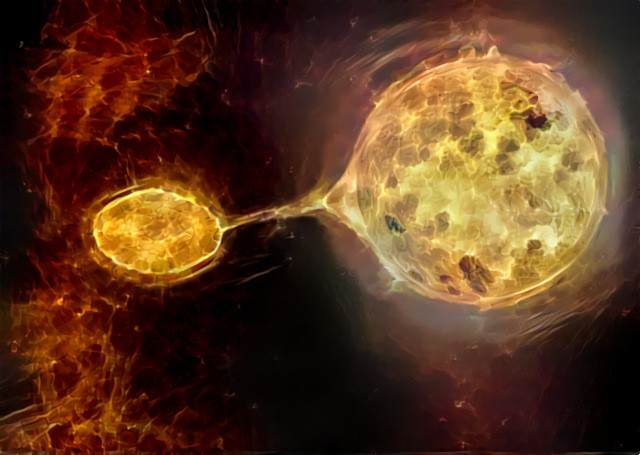
\includegraphics[width=0.75\textwidth]{fig}
  \caption{A figure}
  \label{fig:fig1}
\end{figure}

\subsection{subsection}


%%% Local Variables:
%%% mode:latex
%%% TeX-master: "../../thesis_renzo"
%%% End:
                          % introduction

\chapter[Paper 1]{Paper 1}
\chaptermark{header title} %% if you want a different title in the headers
\label{ch2}

% Define the location of your plots
\graphicspath{{./../gfx/Paper1/}}

% List all paper authors
\chauthors{Your~Name \& Your~Supervisor}
\chjournal{The Astrophysical Journal, 2000, 001, 01}

\begin{abstract}
    \lipsum[1]
\end{abstract}

\section{Introduction}
    \lipsum

\section{Data}
\label{ch:p1:data}
    \lipsum

\section{Results}
    \lipsum

\section{Conclusions} 
    \lipsum
	

%%% Local Variables:
%%% mode: latex
%%% TeX-master: "../../main"
%%% End:

\begin{appendices}
  %   %% modify slightly header defined in styles/layout.tex
  \titleformat{\chapter}[display]{\LARGE}{\vspace*{-2.3\baselineskip}\raggedleft\textcolor{chcol}{\normalsize
      \chaptertitlename\hspace*{4em}}\\\titlerule\vspace*{0.5pc}{\hrulefill\fontsize{150}{150}\selectfont\textcolor{chcol}{\thechapter}}}{-77pt}{ 
    \scshape \rmfamily  \linespread{1000}\parbox[t][0pt][c]{0.8\textwidth}}
  \include{content/chapter2/appendix2} 
\end{appendices}


%%% ---------------------------------------------------------------------------------------
%%%	BIBLIOGRAPHY
%%%------------------------------------------------------------------------------------------
%%% If you disabled the bibliography entry in the TOC my might use this
%%% command to enable a running head.
% \lhead{{\sffamily \small \slshape Bibliography}}

\setlength{\bibsep}{0.0pt}	%%% controls the reference list items separation

%%% Set bibliography styles:
%%% \bibliographystyle{styles/apj} 		%%% apj style, file apj.bst
%%% \bibliographystyle{styles/aa}        %%% A&A style, file aa.bst
\bibliographystyle{styles/linked-apj} 	%%% Customized apj style that recreates ApJ's colored 
					                    %%% hyperlinks to journals [pink] and ADS [blue].
                                        %%% It assumes your bibentries come from ADS, and have

                                        %%% the 'adsurl' keyword.
                                        %%% Do not use this style for print edition!
                                        %%% Do not blindly use this style, it may still have
                                        %%% a few bugs.

								
%%% Load the bibtex library
%%% You can use multiple libraries, but watch out for double entries!
%%% Also make sure that there are no lingering bibliography or style
%%% definitions in the individual chapters. 
\bibliography{content/bibliography/references.bib}


%%%------------------------------------------------------------------------------------------
%%%	BACKMATTER
%%%------------------------------------------------------------------------------------------

%%% The backmatter function turns off chapter numbering
\backmatter
\renewcommand{\chaptermark}[1]{\markboth{\sffamily \small \slshape #1 }{}}  %%% Remove chapter numbering from the headings
%\let\cleardoublepage\clearpage

% !TEX root = ../tex/thesis.tex

% Define a local referenced item command
\newcommand{\coitem}[1]{\item[Chapter~\ref{#1}:] \nameref{#1}}
\newcommand{\coauthors}[1]{\begin{flushleft} {\rm\normalsize #1} \\ \end{flushleft}}
\newcommand{\cojournal}[1]{\begin{flushleft} {\it\normalsize #1} \\ \medskip \end{flushleft}}
\newcommand{\note}[1]{\begin{flushleft} {\footnotesize \normalsize #1} \\ \medskip \end{flushleft}}

% There is no easy way to generate this automatically
\chapter{Contribution from co-authors}
% \vspace*{-1cm}
% \vspace*{1cm}

 \bigskip

\begin{description} 
% This is where you list the contribution of all your coauthors (see article 15 of the regulations).

  \coitem{ch2} %
  \coauthors{you, your co-authors}
  \cojournal{Astronomy \& Astrophysics, 20XX, YY, ZZZ}
  \note{(Also referred to as \citealt{})}
    
\end{description}

%% this is not mandatory
% {
%   \footnotesize
  
%   \noindent The chapters accepted for publication have been typographically
%   adapted.

%   \noindent
%   The following typos have been corrected:
%   \begin{itemize}
%   \item 
%   \end{itemize}
% }


% Reset reference style
\renewcommand\chapterautorefname{chapter}


%%% Local Variables:
%%% mode: latex
%%% TeX-master: "../thesis_renzo"
%%% End:
         %%% mandatory
\chapter[Other publications]{Other publications}

\begin{enumerate}
  \setcounter{enumi}{0}
  \item my other publications
\end{enumerate}

%%% Local Variables:
%%% mode: latex
%%% TeX-master: "../thesis_renzo"
%%% End:
		%%% optional
% !TEX root = ../tex/thesis.tex

% This makes Figure A instead of Figure 1
\renewcommand{\thefigure}{\Alph{figure}}

% This resets the figure counter
\setcounter{figure}{0}

% reset the footnote counter
\setcounter{footnote}{0}

% Set language to Dutch for correct word-breaks.
% It also changes the Figure into Figuur, etc.
\selectlanguage{dutch}
\renewcommand\chapterautorefname{hoofdstuk}%
\cleardoublepage

\chapter{Nederlandse Samenvatting}

\lipsum[6]
 

% Reset language
\selectlanguage{english}
\renewcommand\chapterautorefname{chapter}%


%%% Local Variables:
%%% mode: latex
%%% TeX-master: "../thesis_renzo"
%%% End:
 	    %%% mandatory
%%% \include{content/summary} 		%%% mandatory -- not if it is in the intro!
% !TEX root = ../tex/thesis.tex

\setcounter{footnote}{0}


\chapter{Acknowledgements}


\vspace{10mm}

\raggedleft
Your Name, \\
Date

%%% Local Variables:
%%% mode: latex
%%% TeX-master: "../thesis_renzo"
%%% End:



%% For Ylva: first person I met in AMS
%% For Manos: SNe understanding at 3am in Chicheley Hall
%%  %%% optional (but not really!)
% !TEX root =  thesis.tex

\cleardoublepage
\thispagestyle{empty}
{\raggedright
  \small
  \noindent Ph.D.~thesis, Anton Pannekoek Institute, Universiteit van Amsterdam\\
  \noindent Your Name, Year\\[3ex]

  \noindent ISBN: \todo{N} \\[3ex]


  \noindent Cover design by .\\
  \noindent Credits:
  
  %\noindent The source files for this thesis are available
}



\cleardoublepage
\thispagestyle{empty}
\null\vfill\null

\hfill\parbox{125mm}{ 
\raggedleft\emph{\large afterquote.}\\[5pt]
Someone 
}
\vfill
\clearpage
\thispagestyle{empty}
\newpage
\phantom{let's kill those trees}


\pagestyle{fancy}

%%% Local Variables:
%%% mode: latex
%%% TeX-master: "../thesis_renzo"
%%% End:
        %%% optional
\end{document}

%%% Local Variables:
%%% mode: latex
%%% TeX-master: t
%%% End:
